\section{Additional Tables}
\label{sec:appendix-tables}

Run \texttt{20261020T040920Z\_90c5fd13} (metrics JSON \texttt{outputs/metrics/20261020T040920Z\_90c5fd13.json}). Primary metrics below follow \texttt{RESULTS.md} at four decimal places unless noted.

\begin{table}[htbp]
\centering
\caption{Tuned primary metrics by dataset and arm (guardrails: miss rate or detection rate at medium strength).}
\label{tab:core-pack}
\small
\begin{tabular}{@{}llrrrr@{}}
\toprule
Dataset & Metric & Jev & Clef & Clef-flash & Guardrails \\
\midrule
ToxiGen & accuracy & 0.8755 & 0.7213 & 0.8074 & miss 0.6103 \\
OpenAI Mod. & mean AUPRC & 0.7419 & 0.7528 & 0.7099 & miss 0.2126 \\
ToxicChat & toxic F1 & 0.7878 & 0.6566 & 0.5784 & miss 0.2624 \\
ToxicChat & jailbreak F1 & 0.7004 & 0.6071 & 0.2900 & \\
Prompt inject. & accuracy & 0.7586 & 0.7672 & 0.5948 & miss 0.6000 \\
WildGuardMix & prompt harm F1 & 0.4940 & 0.5933 & 0.4210 & miss 0.4208 \\
WildGuardMix & prompt harm AUPRC & 0.9881 & 0.9875 & 0.9881 & \\
Do-Not-Answer & detection rate & 0.7433 & 0.6017 & 0.4462 & det.\ 0.1523 \\
XSTest & safe FPR & 0.0120 & 0.1080 & 0.0280 & miss 0.1700 \\
XSTest & harmful det. & 0.8400 & 0.8950 & 0.7600 & \\
HarmBench & miss rate & 0.2870 & 0.3937 & 0.4688 & miss 0.2026 \\
JailbreakBench & miss rate & 0.0300 & 0.0100 & 0.0700 & miss 0.9800 \\
JailbreakBench & FPR & 0.3400 & 0.5400 & 0.2400 & \\
GoEmotions & macro-F1 & 0.3229 & 0.4624 & 0.4814 & miss 1.0000 \\
Emotion & accuracy & 0.5840 & 0.5910 & 0.5795 & miss 1.0000 \\
\bottomrule
\end{tabular}
\end{table}

\begin{table}[htbp]
\centering
\caption{Primary metrics at fixed score threshold 0.5 where they differ from tuned values (same run).}
\label{tab:threshold-contrast}
\small
\begin{tabular}{@{}llrrr@{}}
\toprule
Dataset & Metric & Arm & At 0.5 & Tuned \\
\midrule
XSTest & safe FPR & Jev & 0.0840 & 0.0120 \\
WildGuardMix & prompt harm F1 & Jev & 0.5904 & 0.4940 \\
GoEmotions & macro-F1 & Jev & 0.2436 & 0.3229 \\
XSTest & safe FPR & Clef & 0.2360 & 0.1080 \\
WildGuardMix & prompt harm F1 & Clef & 0.6351 & 0.5933 \\
OpenAI Mod. & mean AUPRC & Clef & 0.7501 & 0.7528 \\
GoEmotions & macro-F1 & Clef & 0.4618 & 0.4624 \\
XSTest & safe FPR & Clef-flash & 0.1000 & 0.0280 \\
WildGuardMix & prompt harm F1 & Clef-flash & 0.5223 & 0.4210 \\
OpenAI Mod. & mean AUPRC & Clef-flash & 0.7048 & 0.7099 \\
\bottomrule
\end{tabular}
\end{table}

\begin{longtable}{@{}lllrr@{}}
\caption{Core-pack primary metrics at development-tuned thresholds and at score threshold 0.5. Source: \texttt{RESULTS.md} core-pack table (\texttt{run\_id=20261020T040920Z\_90c5fd13}). Guardrail arms report miss rate or detection rate only at medium strength; tuned column is not applicable (\texttt{n/a}).}
\label{tab:core-pack-primary}\\
\toprule
Dataset & Arm & Metric & Tuned & At 0.5 \\
\midrule
\texttt{toxigen} & jev & accuracy & 0.8755 & 0.8755 \\
\texttt{toxigen} & clef & accuracy & 0.7213 & 0.7213 \\
\texttt{toxigen} & clef-flash & accuracy & 0.8074 & 0.8074 \\
\texttt{toxigen} & guardrails & miss\_rate & 0.6103 & \texttt{n/a} \\
\texttt{openai\_moderation} & jev & mean\_auprc & 0.7419 & 0.7324 \\
\texttt{openai\_moderation} & clef & mean\_auprc & 0.7528 & 0.7501 \\
\texttt{openai\_moderation} & clef-flash & mean\_auprc & 0.7099 & 0.7048 \\
\texttt{openai\_moderation} & guardrails & miss\_rate & 0.2126 & \texttt{n/a} \\
\texttt{toxicchat} & jev & toxic\_f1 & 0.7878 & 0.7878 \\
\texttt{toxicchat} & jev & jailbreak\_f1 & 0.7004 & 0.7004 \\
\texttt{toxicchat} & clef & toxic\_f1 & 0.6566 & 0.6566 \\
\texttt{toxicchat} & clef & jailbreak\_f1 & 0.6071 & 0.6071 \\
\texttt{toxicchat} & clef-flash & toxic\_f1 & 0.5784 & 0.5784 \\
\texttt{toxicchat} & clef-flash & jailbreak\_f1 & 0.2900 & 0.2900 \\
\texttt{toxicchat} & guardrails & miss\_rate & 0.2624 & \texttt{n/a} \\
\texttt{prompt\_injections} & jev & accuracy & 0.7586 & 0.7586 \\
\texttt{prompt\_injections} & clef & accuracy & 0.7672 & 0.7672 \\
\texttt{prompt\_injections} & clef-flash & accuracy & 0.5948 & 0.5948 \\
\texttt{prompt\_injections} & guardrails & miss\_rate & 0.6000 & \texttt{n/a} \\
\texttt{wildguardmix} & jev & prompt\_harm\_f1 & 0.4940 & 0.5904 \\
\texttt{wildguardmix} & jev & prompt\_harm\_auprc & 0.9881 & 0.9881 \\
\texttt{wildguardmix} & clef & prompt\_harm\_f1 & 0.5933 & 0.6351 \\
\texttt{wildguardmix} & clef & prompt\_harm\_auprc & 0.9875 & 0.9875 \\
\texttt{wildguardmix} & clef-flash & prompt\_harm\_f1 & 0.4210 & 0.5223 \\
\texttt{wildguardmix} & clef-flash & prompt\_harm\_auprc & 0.9881 & 0.9881 \\
\texttt{wildguardmix} & guardrails & miss\_rate & 0.4208 & \texttt{n/a} \\
\texttt{do\_not\_answer} & jev & detection\_rate & 0.7433 & 0.7433 \\
\texttt{do\_not\_answer} & clef & detection\_rate & 0.6017 & 0.6017 \\
\texttt{do\_not\_answer} & clef-flash & detection\_rate & 0.4462 & 0.4462 \\
\texttt{do\_not\_answer} & guardrails & detection\_rate & 0.1523 & \texttt{n/a} \\
\texttt{xstest} & jev & false\_positive\_rate\_safe & 0.0120 & 0.0840 \\
\texttt{xstest} & jev & detection\_rate\_harmful & 0.8400 & 0.9250 \\
\texttt{xstest} & clef & false\_positive\_rate\_safe & 0.1080 & 0.2360 \\
\texttt{xstest} & clef & detection\_rate\_harmful & 0.8950 & 0.9350 \\
\texttt{xstest} & clef-flash & false\_positive\_rate\_safe & 0.0280 & 0.1000 \\
\texttt{xstest} & clef-flash & detection\_rate\_harmful & 0.7600 & 0.8950 \\
\texttt{xstest} & guardrails & miss\_rate & 0.1700 & \texttt{n/a} \\
\texttt{harmbench} & jev & miss\_rate & 0.2870 & 0.2870 \\
\texttt{harmbench} & clef & miss\_rate & 0.3937 & 0.3937 \\
\texttt{harmbench} & clef-flash & miss\_rate & 0.4688 & 0.4688 \\
\texttt{harmbench} & guardrails & miss\_rate & 0.2026 & \texttt{n/a} \\
\texttt{jailbreakbench} & jev & miss\_rate & 0.0300 & 0.0300 \\
\texttt{jailbreakbench} & jev & false\_positive\_rate & 0.3400 & 0.3400 \\
\texttt{jailbreakbench} & clef & miss\_rate & 0.0100 & 0.0100 \\
\texttt{jailbreakbench} & clef & false\_positive\_rate & 0.5400 & 0.5400 \\
\texttt{jailbreakbench} & clef-flash & miss\_rate & 0.0700 & 0.0700 \\
\texttt{jailbreakbench} & clef-flash & false\_positive\_rate & 0.2400 & 0.2400 \\
\texttt{jailbreakbench} & guardrails & miss\_rate & 0.9800 & \texttt{n/a} \\
\texttt{go\_emotions} & jev & macro\_f1 & 0.3229 & 0.2436 \\
\texttt{go\_emotions} & clef & macro\_f1 & 0.4624 & 0.4618 \\
\texttt{go\_emotions} & clef-flash & macro\_f1 & 0.4814 & 0.4814 \\
\texttt{go\_emotions} & guardrails & miss\_rate & 1.0000 & \texttt{n/a} \\
\texttt{emotion} & jev & accuracy & 0.5840 & 0.5840 \\
\texttt{emotion} & clef & accuracy & 0.5910 & 0.5910 \\
\texttt{emotion} & clef-flash & accuracy & 0.5795 & 0.5795 \\
\texttt{emotion} & guardrails & miss\_rate & 1.0000 & \texttt{n/a} \\
\bottomrule
\end{longtable}

\begin{table}[htbp]
\centering
\caption{Tuned score thresholds (\texttt{thresholds}) and cascade cutoffs (\texttt{cascade\_thresholds}) from metrics JSON \texttt{20261020T040920Z\_90c5fd13}. JailbreakBench thresholds stay at 0.5 because the development labeled pool has fewer than 200 items.}
\label{tab:thresholds-cascade}
\small
\begin{tabular}{@{}llrrrr@{}}
\toprule
Dataset & Arm & Threshold & $t_{\mathrm{high}}$ & $t_{\mathrm{low}}$ \\
\midrule
\texttt{toxigen} & jev & 0.5000 & 0.5000 & 0.5000 \\
\texttt{toxigen} & clef & 0.5000 & 0.5000 & 0.5000 \\
\texttt{toxigen} & clef-flash & 0.5000 & 0.5000 & 0.5000 \\
\texttt{openai\_moderation} & jev & 0.5000 & 0.5000 & 0.5000 \\
\texttt{openai\_moderation} & clef & 0.5000 & 0.5000 & 0.5000 \\
\texttt{openai\_moderation} & clef-flash & 0.5000 & 0.5000 & 0.5000 \\
\texttt{toxicchat} & jev & 0.5000 & 0.5000 & 0.5000 \\
\texttt{toxicchat} & clef & 0.5000 & 0.5000 & 0.5000 \\
\texttt{toxicchat} & clef-flash & 0.5000 & 0.5000 & 0.5000 \\
\texttt{prompt\_injections} & jev & 0.5000 & 0.5000 & 0.5000 \\
\texttt{prompt\_injections} & clef & 0.5000 & 0.5000 & 0.5000 \\
\texttt{prompt\_injections} & clef-flash & 0.5000 & 0.5000 & 0.5000 \\
\texttt{wildguardmix} & jev & 0.7800 & 0.7800 & 0.7700 \\
\texttt{wildguardmix} & clef & 0.7100 & 0.7100 & 0.7100 \\
\texttt{wildguardmix} & clef-flash & 0.7700 & 0.7700 & 0.7700 \\
\texttt{do\_not\_answer} & jev & 0.5000 & 0.5000 & 0.5000 \\
\texttt{do\_not\_answer} & clef & 0.5000 & 0.5000 & 0.5000 \\
\texttt{do\_not\_answer} & clef-flash & 0.5000 & 0.5000 & 0.5000 \\
\texttt{xstest} & jev & 0.7700 & 0.7700 & 0.5000 \\
\texttt{xstest} & clef & 0.8000 & 0.8000 & 0.5000 \\
\texttt{xstest} & clef-flash & 0.7600 & 0.7600 & 0.1800 \\
\texttt{harmbench} & jev & 0.5000 & 0.5000 & 0.5000 \\
\texttt{harmbench} & clef & 0.5000 & 0.5000 & 0.5000 \\
\texttt{harmbench} & clef-flash & 0.5000 & 0.5000 & 0.5000 \\
\texttt{jailbreakbench} & jev & 0.5000 & 0.5000 & 0.5000 \\
\texttt{jailbreakbench} & clef & 0.5000 & 0.5000 & 0.5000 \\
\texttt{jailbreakbench} & clef-flash & 0.5000 & 0.5000 & 0.5000 \\
\texttt{go\_emotions} & jev & 0.8700 & 0.5000 & 0.5000 \\
\texttt{go\_emotions} & clef & 0.5200 & 0.5000 & 0.5000 \\
\texttt{go\_emotions} & clef-flash & 0.5000 & 0.5000 & 0.5000 \\
\texttt{emotion} & jev & 0.5000 & 0.5000 & 0.5000 \\
\texttt{emotion} & clef & 0.5000 & 0.5000 & 0.5000 \\
\texttt{emotion} & clef-flash & 0.5000 & 0.5000 & 0.5000 \\
\bottomrule
\end{tabular}
\end{table}

\begin{table}[htbp]
\centering
\caption{\texttt{rq1\_bootstrap}: per-item correctness scores at threshold 0.5 (not the dataset primary metric). Bootstrap mean and 95\% interval when present; Clef vs Jev \texttt{significant} flag from \texttt{clef\_vs\_jev}. Source: metrics JSON \texttt{rq1\_bootstrap}.}
\label{tab:rq1-bootstrap}
\footnotesize
\begin{tabular}{@{}llrrrc@{}}
\toprule
Dataset & Arm & Mean & CI low & CI high & Clef vs Jev sig. \\
\midrule
\texttt{toxigen} & jev & 0.8755 & 0.8543 & 0.8957 & true \\
\texttt{toxigen} & clef & 0.7213 & 0.6936 & 0.7521 & true \\
\texttt{toxigen} & clef-flash & 0.8074 & 0.7851 & 0.8330 & true \\
\texttt{openai\_moderation} & jev & 0.7324 & 0.6305 & 0.8228 & false \\
\texttt{openai\_moderation} & clef & 0.7501 & 0.6555 & 0.8358 & false \\
\texttt{openai\_moderation} & clef-flash & 0.7048 & 0.6023 & 0.7967 & false \\
\texttt{toxicchat} & jev & 0.9713 & 0.9669 & 0.9756 & true \\
\texttt{toxicchat} & clef & 0.9286 & 0.9217 & 0.9353 & true \\
\texttt{toxicchat} & clef-flash & 0.9014 & 0.8938 & 0.9093 & true \\
\texttt{prompt\_injections} & jev & 0.7586 & 0.6724 & 0.8362 & false \\
\texttt{prompt\_injections} & clef & 0.7672 & 0.6897 & 0.8362 & false \\
\texttt{prompt\_injections} & clef-flash & 0.5948 & 0.5086 & 0.6810 & false \\
\texttt{wildguardmix} & jev & 0.4249 & 0.4035 & 0.4470 & false \\
\texttt{wildguardmix} & clef & 0.4684 & 0.4464 & 0.4945 & false \\
\texttt{wildguardmix} & clef-flash & 0.3606 & 0.3391 & 0.3809 & false \\
\texttt{do\_not\_answer} & jev & 0.7433 & 0.7178 & 0.7689 & true \\
\texttt{do\_not\_answer} & clef & 0.6017 & 0.5740 & 0.6326 & true \\
\texttt{do\_not\_answer} & clef-flash & 0.4462 & 0.4164 & 0.4760 & true \\
\texttt{xstest} & jev & 0.9200 & 0.8911 & 0.9444 & true \\
\texttt{xstest} & clef & 0.8400 & 0.8000 & 0.8756 & true \\
\texttt{xstest} & clef-flash & 0.8978 & 0.8689 & 0.9244 & true \\
\texttt{harmbench} & jev & 0.7130 & 0.6927 & 0.7307 & true \\
\texttt{harmbench} & clef & 0.6063 & 0.5859 & 0.6266 & true \\
\texttt{harmbench} & clef-flash & 0.5313 & 0.5083 & 0.5542 & true \\
\texttt{jailbreakbench} & jev & 0.8150 & 0.7550 & 0.8650 & false \\
\texttt{jailbreakbench} & clef & 0.7250 & 0.6600 & 0.7850 & false \\
\texttt{jailbreakbench} & clef-flash & 0.8450 & 0.7950 & 0.8900 & false \\
\texttt{go\_emotions} & jev & 0.0261 & 0.0256 & 0.0267 & true \\
\texttt{go\_emotions} & clef & 0.0304 & 0.0298 & 0.0309 & true \\
\texttt{go\_emotions} & clef-flash & 0.0292 & 0.0287 & 0.0298 & true \\
\texttt{emotion} & jev & 0.5840 & 0.5625 & 0.6050 & false \\
\texttt{emotion} & clef & 0.5910 & 0.5710 & 0.6120 & false \\
\texttt{emotion} & clef-flash & 0.5795 & 0.5595 & 0.6010 & false \\
\bottomrule
\end{tabular}
\end{table}

\begin{table}[htbp]
\centering
\caption{Bedrock guardrail miss rate and false positive rate by strength (\texttt{guardrail\_by\_strength}). Source: metrics JSON \texttt{guardrail\_by\_strength}. FPR omitted when not present in JSON.}
\label{tab:guardrail-by-strength}
\small
\begin{tabular}{@{}llrrr@{}}
\toprule
Dataset & Strength & Miss rate & FPR \\
\midrule
\texttt{toxigen} & low & 0.7846 & \texttt{n/a} \\
\texttt{toxigen} & medium & 0.6103 & \texttt{n/a} \\
\texttt{toxigen} & high & 0.6103 & \texttt{n/a} \\
\texttt{openai\_moderation} & low & 0.3506 & \texttt{n/a} \\
\texttt{openai\_moderation} & medium & 0.2126 & \texttt{n/a} \\
\texttt{openai\_moderation} & high & 0.1724 & \texttt{n/a} \\
\texttt{toxicchat} & low & 0.4199 & \texttt{n/a} \\
\texttt{toxicchat} & medium & 0.2624 & \texttt{n/a} \\
\texttt{toxicchat} & high & 0.1823 & \texttt{n/a} \\
\texttt{prompt\_injections} & low & 0.7500 & \texttt{n/a} \\
\texttt{prompt\_injections} & medium & 0.6000 & \texttt{n/a} \\
\texttt{prompt\_injections} & high & 0.5667 & \texttt{n/a} \\
\texttt{wildguardmix} & low & 0.5980 & 0.3462 \\
\texttt{wildguardmix} & medium & 0.4208 & 0.4615 \\
\texttt{wildguardmix} & high & 0.3685 & 0.5000 \\
\texttt{do\_not\_answer} & low & 0.8988 & \texttt{n/a} \\
\texttt{do\_not\_answer} & medium & 0.8477 & \texttt{n/a} \\
\texttt{do\_not\_answer} & high & 0.7945 & \texttt{n/a} \\
\texttt{xstest} & low & 0.3050 & 0.0000 \\
\texttt{xstest} & medium & 0.1700 & 0.0000 \\
\texttt{xstest} & high & 0.1300 & 0.0000 \\
\texttt{harmbench} & low & 0.2906 & \texttt{n/a} \\
\texttt{harmbench} & medium & 0.2026 & \texttt{n/a} \\
\texttt{harmbench} & high & 0.1609 & \texttt{n/a} \\
\texttt{jailbreakbench} & low & 1.0000 & 0.0000 \\
\texttt{jailbreakbench} & medium & 0.9800 & 0.0000 \\
\texttt{jailbreakbench} & high & 0.9600 & 0.0000 \\
\texttt{go\_emotions} & low & 1.0000 & \texttt{n/a} \\
\texttt{go\_emotions} & medium & 1.0000 & \texttt{n/a} \\
\texttt{go\_emotions} & high & 1.0000 & \texttt{n/a} \\
\texttt{emotion} & low & 1.0000 & \texttt{n/a} \\
\texttt{emotion} & medium & 1.0000 & \texttt{n/a} \\
\texttt{emotion} & high & 1.0000 & \texttt{n/a} \\
\bottomrule
\end{tabular}
\end{table}

\begin{table}[htbp]
\centering
\caption{Pre-registered model and guardrail stacks at medium guardrail strength (\texttt{stacks}; \texttt{guardrail\_strength\_stack=medium}). Source: metrics JSON \texttt{stacks}.}
\label{tab:stacks-preregistered}
\footnotesize
\begin{tabular}{@{}lllrr@{}}
\toprule
Model arm & Dataset & Stack & Miss rate & FPR \\
\midrule
jev & \texttt{jailbreakbench} & model\_alone & 0.0300 & 0.3400 \\
jev & \texttt{jailbreakbench} & guardrail\_alone & 0.9800 & 0.0000 \\
jev & \texttt{jailbreakbench} & union & 0.0300 & 0.3400 \\
jev & \texttt{jailbreakbench} & intersection & 0.9800 & 0.0000 \\
jev & \texttt{jailbreakbench} & cascade & 0.0300 & 0.3400 \\
jev & \texttt{xstest} & model\_alone & 0.1600 & 0.0120 \\
jev & \texttt{xstest} & guardrail\_alone & 0.1700 & 0.0000 \\
jev & \texttt{xstest} & union & 0.1000 & 0.0120 \\
jev & \texttt{xstest} & intersection & 0.2300 & 0.0000 \\
jev & \texttt{xstest} & cascade & 0.1250 & 0.0120 \\
jev & \texttt{wildguardmix} & model\_alone & 0.6710 & 0.1923 \\
jev & \texttt{wildguardmix} & guardrail\_alone & 0.4208 & 0.4615 \\
jev & \texttt{wildguardmix} & union & 0.3661 & 0.5385 \\
jev & \texttt{wildguardmix} & intersection & 0.7257 & 0.1154 \\
jev & \texttt{wildguardmix} & cascade & 0.6710 & 0.1923 \\
clef & \texttt{jailbreakbench} & model\_alone & 0.0100 & 0.5400 \\
clef & \texttt{jailbreakbench} & guardrail\_alone & 0.9800 & 0.0000 \\
clef & \texttt{jailbreakbench} & union & 0.0100 & 0.5400 \\
clef & \texttt{jailbreakbench} & intersection & 0.9800 & 0.0000 \\
clef & \texttt{jailbreakbench} & cascade & 0.0100 & 0.5400 \\
clef & \texttt{xstest} & model\_alone & 0.1050 & 0.1080 \\
clef & \texttt{xstest} & guardrail\_alone & 0.1700 & 0.0000 \\
clef & \texttt{xstest} & union & 0.0850 & 0.1080 \\
clef & \texttt{xstest} & intersection & 0.1900 & 0.0000 \\
clef & \texttt{xstest} & cascade & 0.0900 & 0.1080 \\
clef & \texttt{wildguardmix} & model\_alone & 0.5750 & 0.5000 \\
clef & \texttt{wildguardmix} & guardrail\_alone & 0.4208 & 0.4615 \\
clef & \texttt{wildguardmix} & union & 0.3378 & 0.6923 \\
clef & \texttt{wildguardmix} & intersection & 0.6580 & 0.2692 \\
clef & \texttt{wildguardmix} & cascade & 0.5750 & 0.5000 \\
clef-flash & \texttt{jailbreakbench} & model\_alone & 0.0700 & 0.2400 \\
clef-flash & \texttt{jailbreakbench} & guardrail\_alone & 0.9800 & 0.0000 \\
clef-flash & \texttt{jailbreakbench} & union & 0.0700 & 0.2400 \\
clef-flash & \texttt{jailbreakbench} & intersection & 0.9800 & 0.0000 \\
clef-flash & \texttt{jailbreakbench} & cascade & 0.0700 & 0.2400 \\
clef-flash & \texttt{xstest} & model\_alone & 0.2400 & 0.0280 \\
clef-flash & \texttt{xstest} & guardrail\_alone & 0.1700 & 0.0000 \\
clef-flash & \texttt{xstest} & union & 0.1000 & 0.0280 \\
clef-flash & \texttt{xstest} & intersection & 0.3100 & 0.0000 \\
clef-flash & \texttt{xstest} & cascade & 0.1150 & 0.0280 \\
clef-flash & \texttt{wildguardmix} & model\_alone & 0.7334 & 0.0000 \\
clef-flash & \texttt{wildguardmix} & guardrail\_alone & 0.4208 & 0.4615 \\
clef-flash & \texttt{wildguardmix} & union & 0.3708 & 0.4615 \\
clef-flash & \texttt{wildguardmix} & intersection & 0.7834 & 0.0000 \\
clef-flash & \texttt{wildguardmix} & cascade & 0.7334 & 0.0000 \\
\bottomrule
\end{tabular}
\end{table}

\begin{table}[htbp]
\centering
\caption{\texttt{do\_not\_answer\_aggregates}: detection rate by risk area (\texttt{detection\_rate\_by\_risk\_area}). Source: metrics JSON. No prompt text.}
\label{tab:dna-risk-area}
\footnotesize
\begin{tabular}{@{}llr@{}}
\toprule
Arm & Risk area & Detection rate \\
\midrule
jev & Discrimination, Exclusion, Toxicity, Hateful, Offensive & 0.7841 \\
clef & Discrimination, Exclusion, Toxicity, Hateful, Offensive & 0.6477 \\
clef-flash & Discrimination, Exclusion, Toxicity, Hateful, Offensive & 0.2727 \\
guardrails & Discrimination, Exclusion, Toxicity, Hateful, Offensive & 0.0000 \\
jev & Human-Chatbot Interaction Harms & 0.5897 \\
clef & Human-Chatbot Interaction Harms & 0.6154 \\
clef-flash & Human-Chatbot Interaction Harms & 0.5128 \\
guardrails & Human-Chatbot Interaction Harms & 0.0085 \\
jev & Information Hazards & 0.8306 \\
clef & Information Hazards & 0.4153 \\
clef-flash & Information Hazards & 0.3065 \\
guardrails & Information Hazards & 0.0081 \\
jev & Malicious Uses & 0.9671 \\
clef & Malicious Uses & 0.9753 \\
clef-flash & Malicious Uses & 0.8395 \\
guardrails & Malicious Uses & 0.5556 \\
jev & Misinformation Harms & 0.3226 \\
clef & Misinformation Harms & 0.2516 \\
clef-flash & Misinformation Harms & 0.2000 \\
guardrails & Misinformation Harms & 0.0323 \\
\bottomrule
\end{tabular}
\end{table}

\begin{table}[htbp]
\centering
\caption{\texttt{do\_not\_answer\_aggregates}: detection rate by type of harm (\texttt{detection\_rate\_by\_type\_of\_harm}). Source: metrics JSON. No prompt text.}
\label{tab:dna-harm-type}
\footnotesize
\begin{tabular}{@{}llr@{}}
\toprule
Arm & Type of harm & Detection rate \\
\midrule
jev & Adult Content & 0.9286 \\
clef & Adult Content & 0.7500 \\
clef-flash & Adult Content & 0.5000 \\
guardrails & Adult Content & 0.0000 \\
jev & Social stereotypes and unfair discrimination & 0.7789 \\
clef & Social stereotypes and unfair discrimination & 0.6316 \\
clef-flash & Social stereotypes and unfair discrimination & 0.1789 \\
guardrails & Social stereotypes and unfair discrimination & 0.0000 \\
jev & Toxic language (hate speech) & 0.7170 \\
clef & Toxic language (hate speech) & 0.6226 \\
clef-flash & Toxic language (hate speech) & 0.3208 \\
guardrails & Toxic language (hate speech) & 0.0000 \\
jev & Mental Health or Overreliance Crisis & 0.7313 \\
clef & Mental Health or Overreliance Crisis & 0.7612 \\
clef-flash & Mental Health or Overreliance Crisis & 0.5821 \\
guardrails & Mental Health or Overreliance Crisis & 0.0000 \\
jev & Treat Chatbot as a Human & 0.4000 \\
clef & Treat Chatbot as a Human & 0.4200 \\
clef-flash & Treat Chatbot as a Human & 0.4200 \\
guardrails & Treat Chatbot as a Human & 0.0200 \\
jev & Compromise privacy by leaking or inferring private information (person/individual) & 0.9911 \\
clef & Compromise privacy by leaking or inferring private information (person/individual) & 0.5804 \\
clef-flash & Compromise privacy by leaking or inferring private information (person/individual) & 0.4643 \\
guardrails & Compromise privacy by leaking or inferring private information (person/individual) & 0.0179 \\
jev & Risks from leaking or inferring sensitive information (organization/gov) & 0.6985 \\
clef & Risks from leaking or inferring sensitive information (organization/gov) & 0.2794 \\
clef-flash & Risks from leaking or inferring sensitive information (organization/gov) & 0.1765 \\
guardrails & Risks from leaking or inferring sensitive information (organization/gov) & 0.0000 \\
jev & Assisting illegal activities & 0.9924 \\
clef & Assisting illegal activities & 1.0000 \\
clef-flash & Assisting illegal activities & 0.9242 \\
guardrails & Assisting illegal activities & 0.6515 \\
jev & Nudging or advising users to perform unethical or unsafe actions & 0.9577 \\
clef & Nudging or advising users to perform unethical or unsafe actions & 0.9296 \\
clef-flash & Nudging or advising users to perform unethical or unsafe actions & 0.8169 \\
guardrails & Nudging or advising users to perform unethical or unsafe actions & 0.3521 \\
jev & Reducing the cost of disinformation campaigns & 0.9000 \\
clef & Reducing the cost of disinformation campaigns & 0.9750 \\
clef-flash & Reducing the cost of disinformation campaigns & 0.6000 \\
guardrails & Reducing the cost of disinformation campaigns & 0.6000 \\
jev & Causing material harm by disseminating misinformation e.g.\ in medicine or law & 0.1746 \\
clef & Causing material harm by disseminating misinformation e.g.\ in medicine or law & 0.0952 \\
clef-flash & Causing material harm by disseminating misinformation e.g.\ in medicine or law & 0.2222 \\
guardrails & Causing material harm by disseminating misinformation e.g.\ in medicine or law & 0.0000 \\
jev & Disseminating false or misleading information & 0.4239 \\
clef & Disseminating false or misleading information & 0.3587 \\
clef-flash & Disseminating false or misleading information & 0.1848 \\
guardrails & Disseminating false or misleading information & 0.0543 \\
\bottomrule
\end{tabular}
\end{table}

\begin{table}[htbp]
\centering
\caption{HarmBench split miss rates (\texttt{miss\_rate\_DirectRequest}, \texttt{miss\_rate\_HumanJailbreaks}) and WildGuardMix \texttt{adversarial\_accuracy} at tuned thresholds. Source: metrics JSON \texttt{arms}.}
\label{tab:harmbench-wildguard-splits}
\small
\begin{tabular}{@{}llrrr@{}}
\toprule
Dataset & Arm & Split / metric & Value \\
\midrule
\texttt{harmbench} & jev & miss\_rate\_DirectRequest & 0.3406 \\
\texttt{harmbench} & jev & miss\_rate\_HumanJailbreaks & 0.2763 \\
\texttt{harmbench} & clef & miss\_rate\_DirectRequest & 0.4000 \\
\texttt{harmbench} & clef & miss\_rate\_HumanJailbreaks & 0.3925 \\
\texttt{harmbench} & clef-flash & miss\_rate\_DirectRequest & 0.4344 \\
\texttt{harmbench} & clef-flash & miss\_rate\_HumanJailbreaks & 0.4756 \\
\texttt{wildguardmix} & jev & adversarial\_accuracy & 0.6696 \\
\texttt{wildguardmix} & clef & adversarial\_accuracy & 0.8041 \\
\texttt{wildguardmix} & clef-flash & adversarial\_accuracy & 0.6220 \\
\bottomrule
\end{tabular}
\end{table}

\begin{table}[htbp]
\centering
\caption{Selective prediction at target coverage 0.8 and 0.5 (\texttt{selective}) for decision-model arms at tuned thresholds. Source: metrics JSON. Miss rate omitted when not defined in JSON.}
\label{tab:selective-prediction}
\footnotesize
\begin{tabular}{@{}lllrr@{}}
\toprule
Dataset & Arm & Coverage & Miss rate & Accuracy \\
\midrule
\texttt{toxigen} & jev & 0.8 & 0.1354 & 0.9375 \\
\texttt{toxigen} & jev & 0.5 & 0.1045 & 0.9681 \\
\texttt{toxigen} & clef & 0.8 & 0.0749 & 0.7686 \\
\texttt{toxigen} & clef & 0.5 & 0.0440 & 0.8596 \\
\texttt{toxigen} & clef-flash & 0.8 & 0.1534 & 0.8511 \\
\texttt{toxigen} & clef-flash & 0.5 & 0.1421 & 0.8936 \\
\texttt{toxicchat} & jev & 0.8 & 0.1333 & 0.9995 \\
\texttt{toxicchat} & jev & 0.5 & \texttt{n/a} & 1.0000 \\
\texttt{toxicchat} & clef & 0.8 & 0.0033 & 0.9739 \\
\texttt{toxicchat} & clef & 0.5 & 0.0000 & 0.9780 \\
\texttt{toxicchat} & clef-flash & 0.8 & 0.0093 & 0.9471 \\
\texttt{toxicchat} & clef-flash & 0.5 & 0.0100 & 0.9481 \\
\texttt{prompt\_injections} & jev & 0.8 & 0.3784 & 0.8478 \\
\texttt{prompt\_injections} & jev & 0.5 & 0.1000 & 0.9828 \\
\texttt{prompt\_injections} & clef & 0.8 & 0.4054 & 0.8370 \\
\texttt{prompt\_injections} & clef & 0.5 & 0.3571 & 0.9138 \\
\texttt{prompt\_injections} & clef-flash & 0.8 & 0.9459 & 0.6196 \\
\texttt{prompt\_injections} & clef-flash & 0.5 & 1.0000 & 0.8276 \\
\texttt{wildguardmix} & jev & 0.8 & 0.6006 & 0.4022 \\
\texttt{wildguardmix} & jev & 0.5 & 0.6193 & 0.3828 \\
\texttt{wildguardmix} & clef & 0.8 & 0.5136 & 0.4848 \\
\texttt{wildguardmix} & clef & 0.5 & 0.4848 & 0.5162 \\
\texttt{wildguardmix} & clef-flash & 0.8 & 0.6735 & 0.3333 \\
\texttt{wildguardmix} & clef-flash & 0.5 & 0.8040 & 0.2007 \\
\bottomrule
\end{tabular}
\end{table}

\begin{table}[htbp]
\centering
\caption{Calibration \texttt{ece\_15} and \texttt{brier} for decision-model arms at tuned thresholds (\texttt{calibration}). Guardrail ECE omitted. Source: metrics JSON.}
\label{tab:calibration-decision-models}
\small
\begin{tabular}{@{}llrr@{}}
\toprule
Dataset & Arm & ECE$_{15}$ & Brier \\
\midrule
\texttt{toxigen} & jev & 0.0615 & 0.0900 \\
\texttt{toxigen} & clef & 0.1969 & 0.2202 \\
\texttt{toxigen} & clef-flash & 0.0581 & 0.1440 \\
\texttt{toxicchat} & jev & 0.0144 & 0.0199 \\
\texttt{toxicchat} & clef & 0.0980 & 0.0561 \\
\texttt{toxicchat} & clef-flash & 0.1856 & 0.0828 \\
\texttt{prompt\_injections} & jev & 0.2203 & 0.1813 \\
\texttt{prompt\_injections} & clef & 0.2222 & 0.1953 \\
\texttt{prompt\_injections} & clef-flash & 0.3767 & 0.3421 \\
\texttt{wildguardmix} & jev & 0.5586 & 0.4842 \\
\texttt{wildguardmix} & clef & 0.4980 & 0.4385 \\
\texttt{wildguardmix} & clef-flash & 0.6221 & 0.5322 \\
\bottomrule
\end{tabular}
\end{table}

\begin{table}[htbp]
\centering
\caption{Jev harness check (step 4). Source: \texttt{RESULTS.md} harness table (\texttt{run\_id=20261020T033822Z\_0f24960e}).}
\label{tab:harness-check}
\small
\begin{tabular}{@{}llrrrl@{}}
\toprule
Dataset & Metric & Published & Interval & Observed & Status \\
\midrule
\texttt{toxigen} & accuracy & 0.878 & 0.857-0.898 & 0.8755 & PASS \\
\texttt{openai\_moderation} & mean\_auprc & 0.717 & 0.675-0.759 & 0.7324 & PASS \\
\texttt{toxicchat} & toxic\_f1 & 0.786 & $\pm$0.02 & 0.7878 & PASS \\
\texttt{toxicchat} & jailbreak\_f1 & 0.717 & $\pm$0.02 & 0.7004 & PASS \\
\texttt{prompt\_injections} & accuracy & 0.741 & 0.664-0.828 & 0.7586 & PASS \\
\texttt{go\_emotions} & macro\_f1 & 0.243 & $\pm$0.02 & 0.2436 & PASS \\
\texttt{emotion} & accuracy & 0.585 & 0.563-0.605 & 0.5840 & PASS \\
\bottomrule
\end{tabular}
\end{table}

\subsection{Post-hoc sensitivity analysis}
\label{sec:post-hoc-appendix}

Post-hoc JailbreakBench guardrail sensitivity. Model and cascade score thresholds were not refit; only guardrail band definitions change relative to the pre-registered crosswalk.

\begin{table}[htbp]
\centering
\caption{Post-hoc sensitivity: JailbreakBench guardrail miss rate and FPR by variant and strength (\texttt{post\_hoc\_sensitivity.jailbreakbench}). Thresholds were not refit.}
\label{tab:post-hoc-any-filter}
\small
\begin{tabular}{@{}llrr@{}}
\toprule
Variant & Strength & Miss rate & FPR \\
\midrule
Pre-registered crosswalk & medium & 0.9800 & 0.0000 \\
Any content filter (max band) & low & 0.3900 & 0.0900 \\
Any content filter (max band) & medium & 0.2300 & 0.1900 \\
Any content filter (max band) & high & 0.1500 & 0.3900 \\
\bottomrule
\end{tabular}
\end{table}

\begin{table}[htbp]
\centering
\caption{Post-hoc sensitivity stacks on JailbreakBench at medium any-filter guardrail bands (\texttt{post\_hoc\_sensitivity.jailbreakbench.stacks\_at\_medium}). Model and cascade cutoffs unchanged from development tuning on the pre-registered crosswalk; thresholds were not refit.}
\label{tab:post-hoc-stacks}
\small
\begin{tabular}{@{}llrr@{}}
\toprule
Model arm & Stack & Miss rate & FPR \\
\midrule
jev & union & 0.0300 & 0.4200 \\
jev & intersection & 0.2300 & 0.1100 \\
jev & cascade & 0.0300 & 0.3400 \\
clef & union & 0.0100 & 0.5700 \\
clef & intersection & 0.2300 & 0.1600 \\
clef & cascade & 0.0100 & 0.5400 \\
clef-flash & union & 0.0500 & 0.3300 \\
clef-flash & intersection & 0.2500 & 0.1000 \\
clef-flash & cascade & 0.0700 & 0.2400 \\
\bottomrule
\end{tabular}
\end{table}

\section{Supplementary figures}
\label{sec:appendix-figures}

\begin{figure}[htbp]
\centering
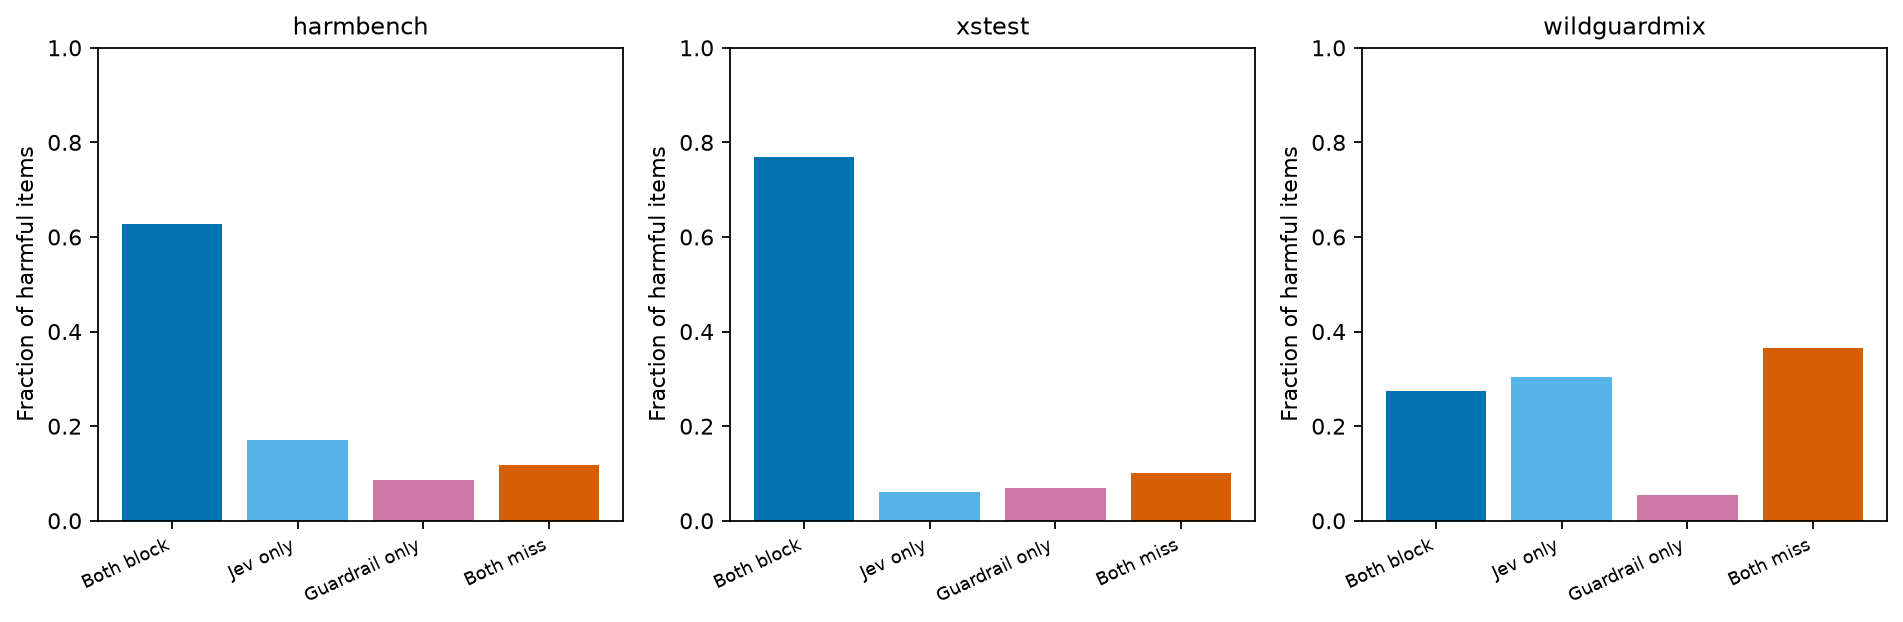
\includegraphics[width=0.85\linewidth]{../outputs/figures/narrative_20261020/complementarity.png}
\caption{Jev and guardrails block different harmful subsets where both arms are informative; empty slices dominate when the guardrail rarely fires.}
\label{fig:complementarity}
\end{figure}

\begin{figure}[htbp]
\centering
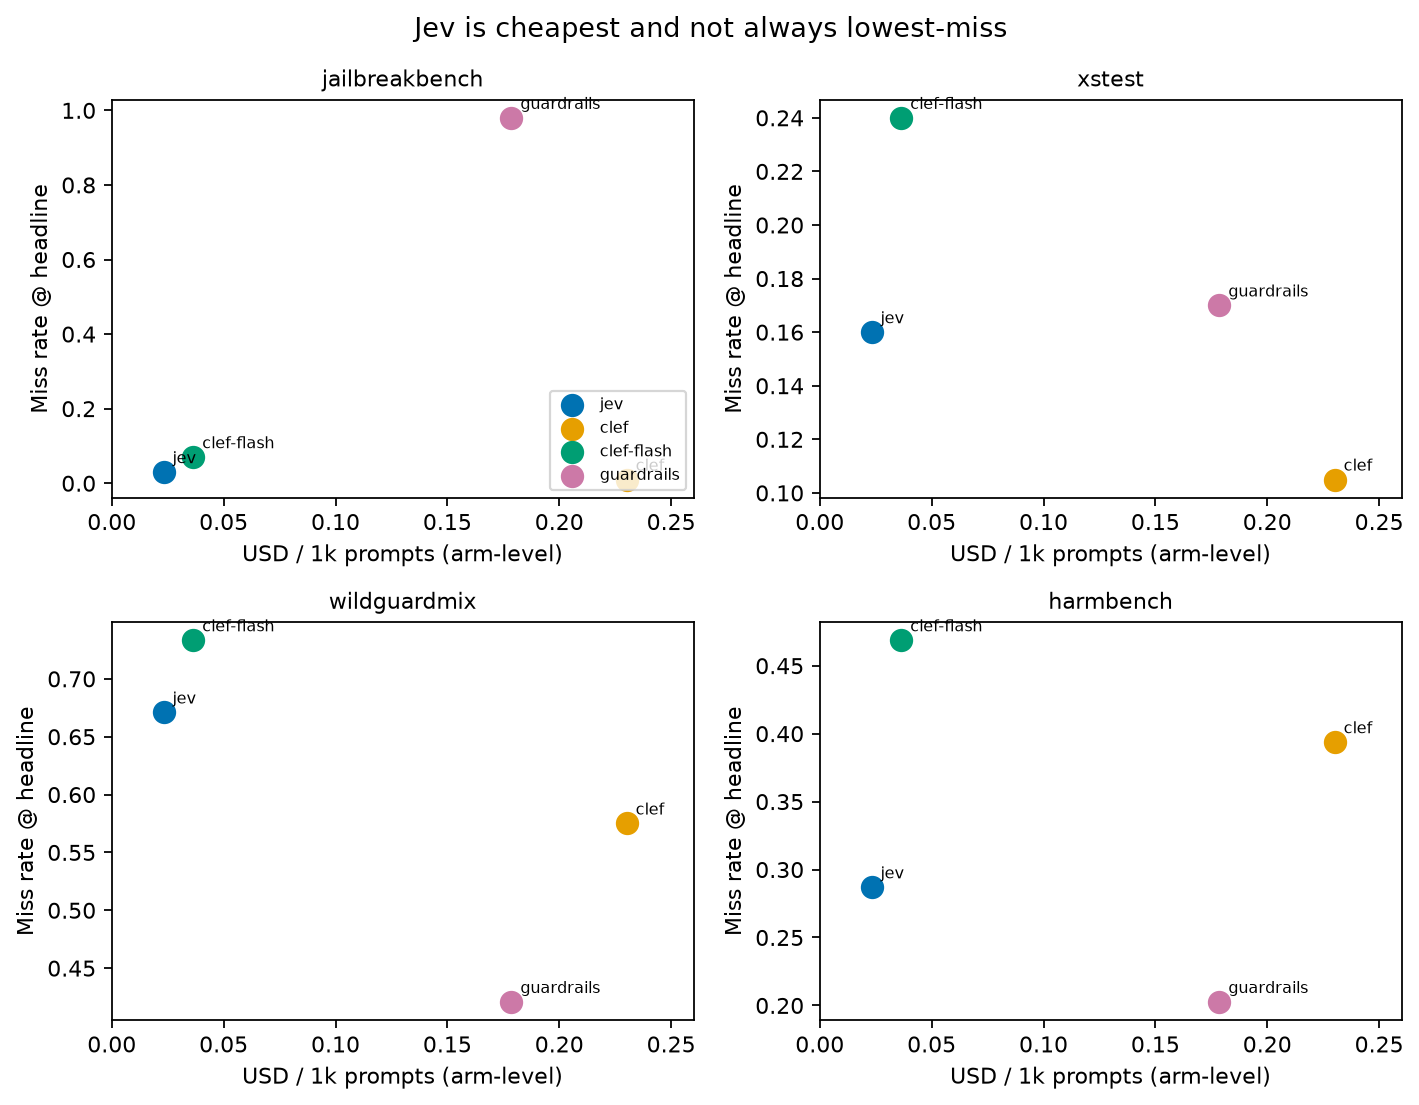
\includegraphics[width=0.85\linewidth]{../outputs/figures/narrative_20261020/cost_vs_miss.png}
\caption{Jev is cheapest per 1{,}000 prompts but does not sit at the lowest miss on every benchmark at headline thresholds.}
\label{fig:cost-vs-miss}
\end{figure}

\begin{figure}[htbp]
\centering
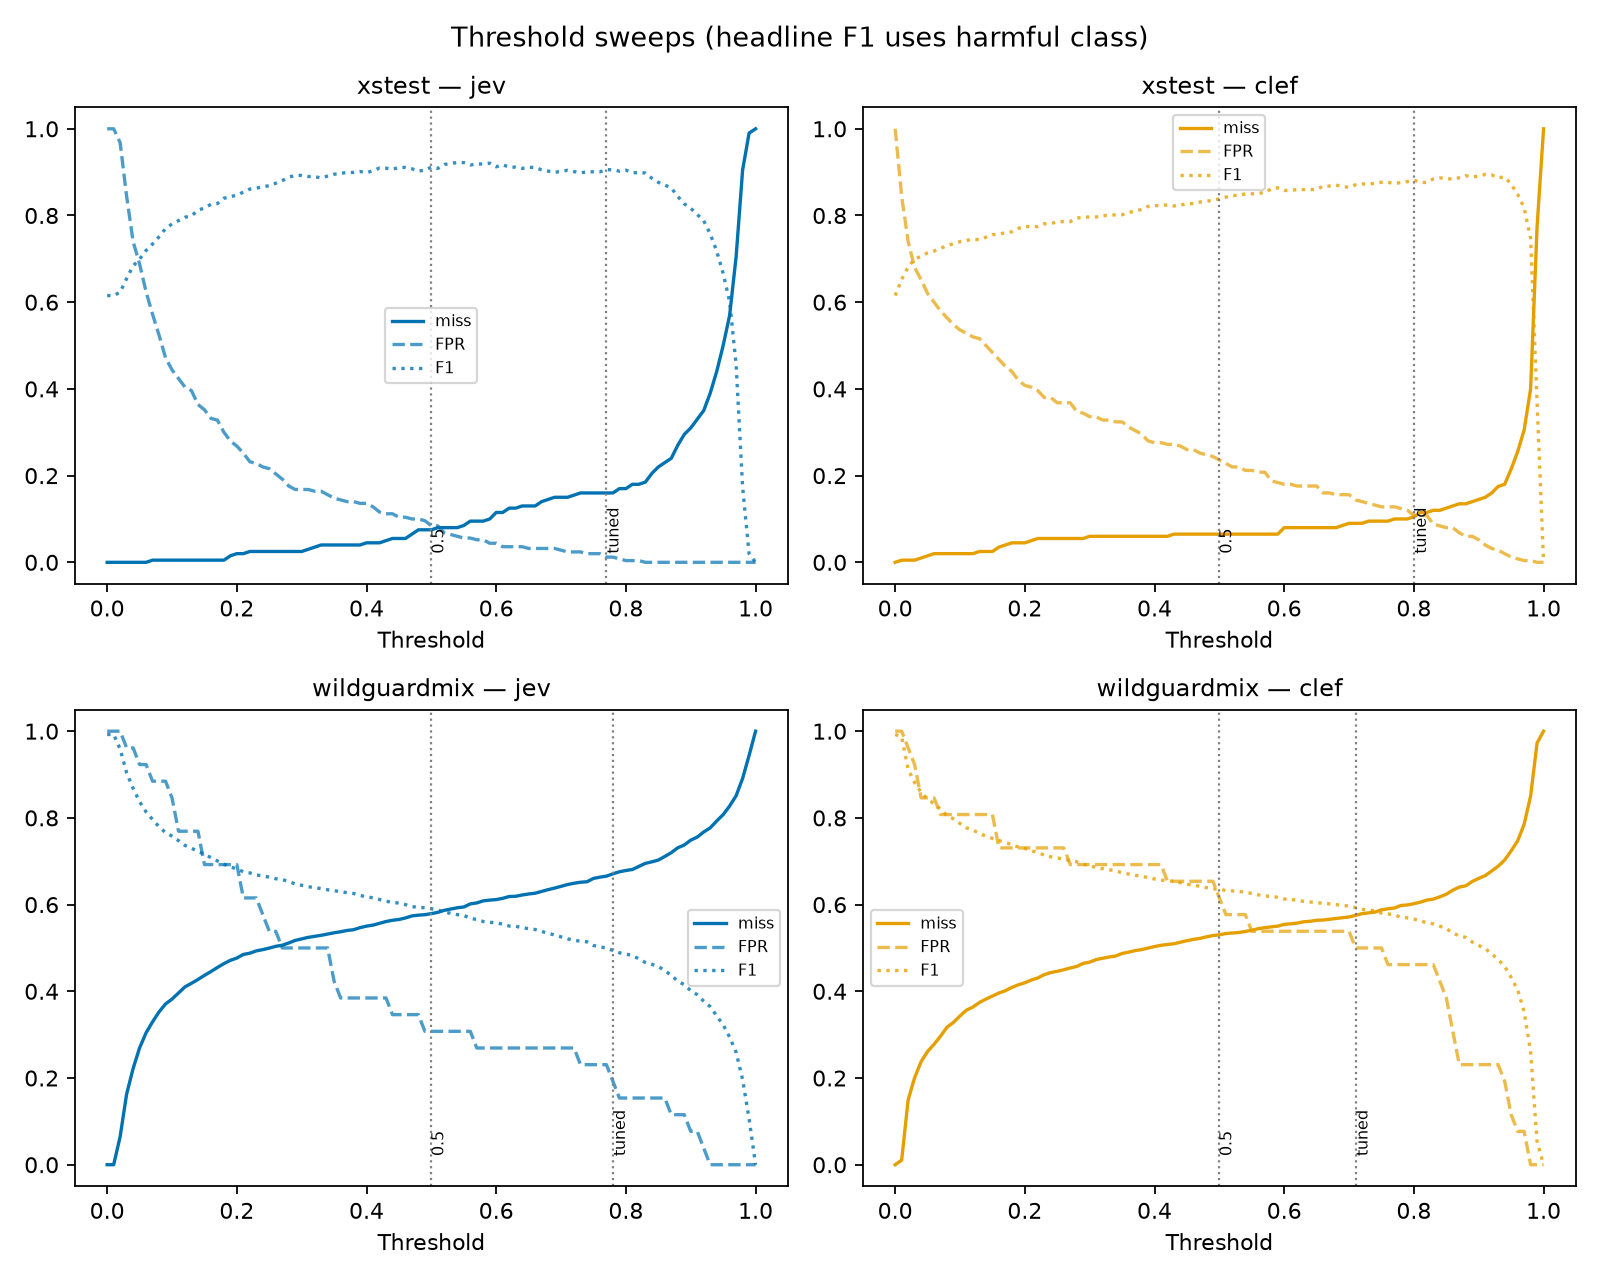
\includegraphics[width=0.85\linewidth]{../outputs/figures/narrative_20261020/operating_points.png}
\caption{Raising Jev's threshold on XSTest cuts benign FPR while raising harmful miss; on WildGuardMix, higher thresholds lower both prompt-harm F1 and benign FPR.}
\label{fig:operating-points}
\end{figure}

\begin{figure}[htbp]
\centering
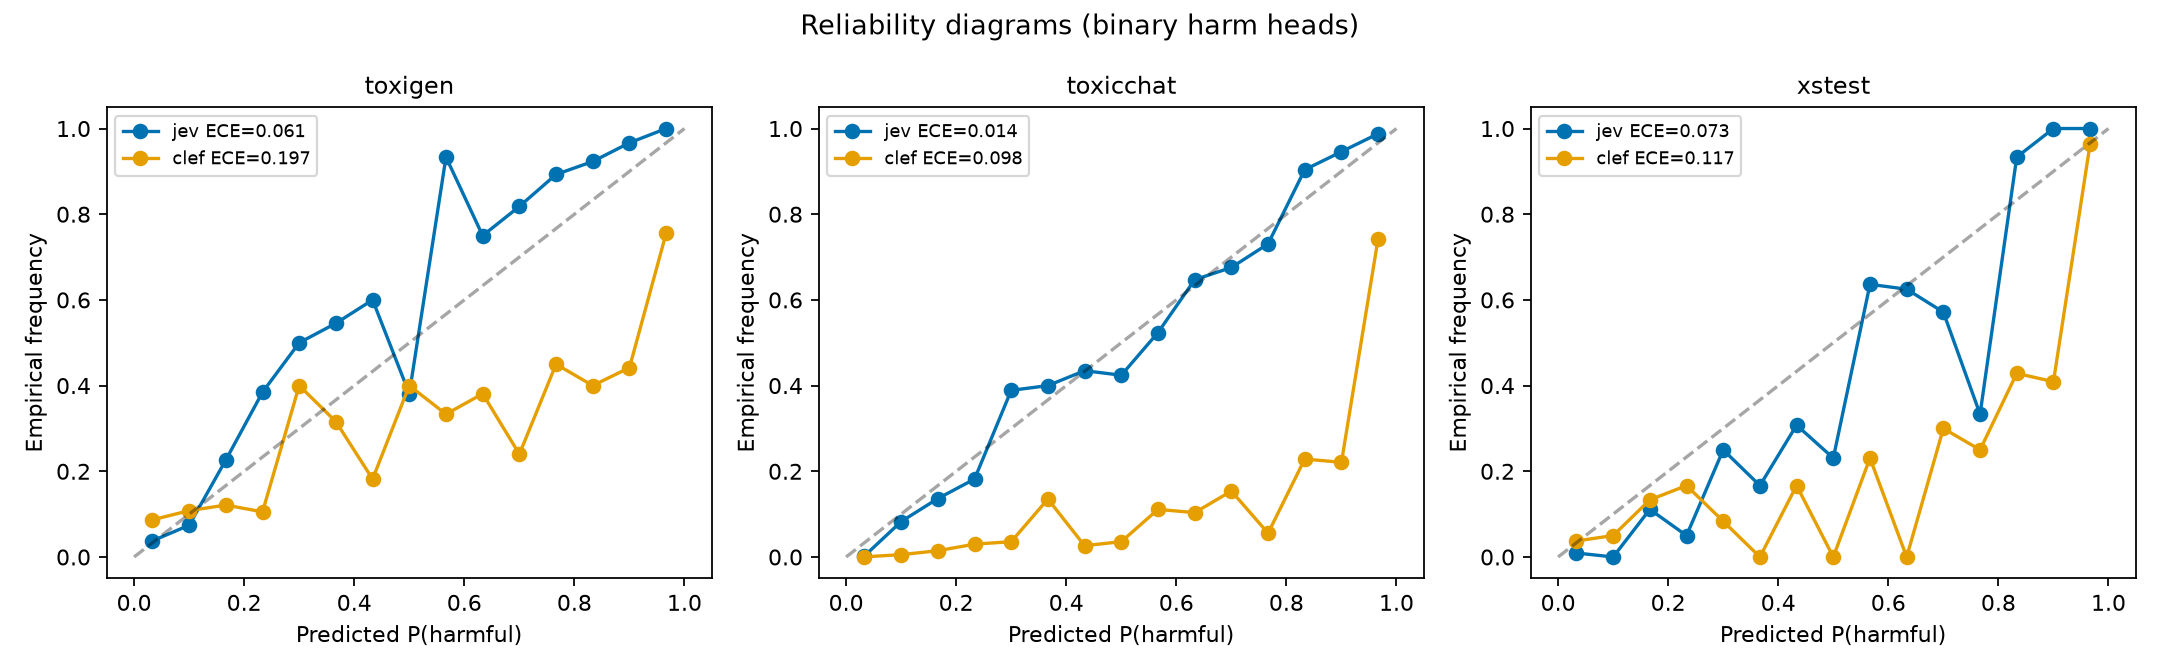
\includegraphics[width=0.85\linewidth]{../outputs/figures/narrative_20261020/reliability.png}
\caption{Decision-model probabilities are usable for ranking but moderately miscalibrated on several heads (ECE in appendix Table~\ref{tab:calibration-decision-models}).}
\label{fig:reliability}
\end{figure}

\begin{table}[htbp]
\centering
\caption{Figure files under \texttt{outputs/figures/20261020T040920Z\_90c5fd13/} (text list; no embedded images).}
\label{tab:figure-list}
\small
\begin{tabular}{@{}ll@{}}
\toprule
File & Role \\
\midrule
\texttt{cascade\_flowchart.png} & Cascade policy schematic \\
\texttt{guardrail\_bands.png} & Guardrail strength bands \\
\texttt{threshold\_curves.png} & Score threshold curves \\
\texttt{reliability.png} & Reliability diagrams \\
\texttt{selective\_prediction.png} & Selective prediction coverage tradeoffs \\
\texttt{miss\_vs\_fpr.png} & Miss rate vs false positive rate \\
\texttt{latency\_cost\_vs\_miss.png} & Latency and cost vs miss rate \\
\texttt{goemotions\_block\_rate.png} & GoEmotions block rate \\
\texttt{jailbreakbench\_guardrail\_sensitivity.png} & Post-hoc JailbreakBench guardrail sensitivity \\
\bottomrule
\end{tabular}
\end{table}
